\newpage
\mysubsection{Cache}

%--  \begin{figure}[hb]
%--    \begin{center}
%--      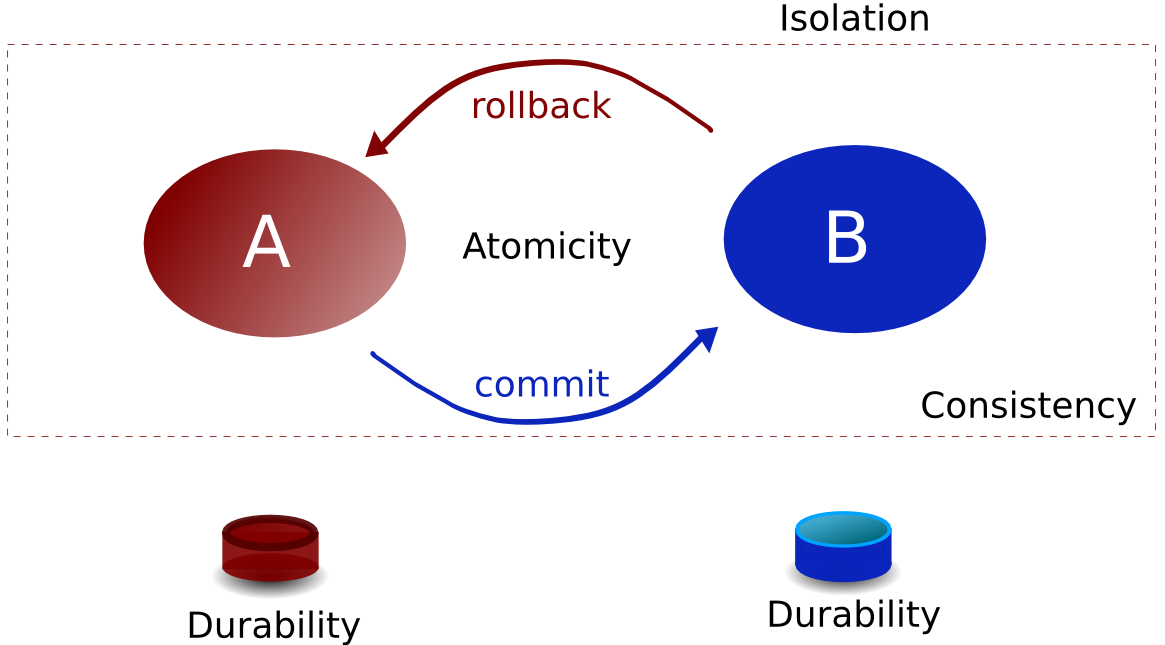
\includegraphics[scale=0.4]{img/transaction.png}
%--      \caption{Caractéristique d'une transaction}
%--      \label{tx}
%--    \end{center}
%--  \end{figure}
%--}
%--
%--\ifslide{
%--  \begin{frame}{Transaction}
%--   \begin{center}
%--     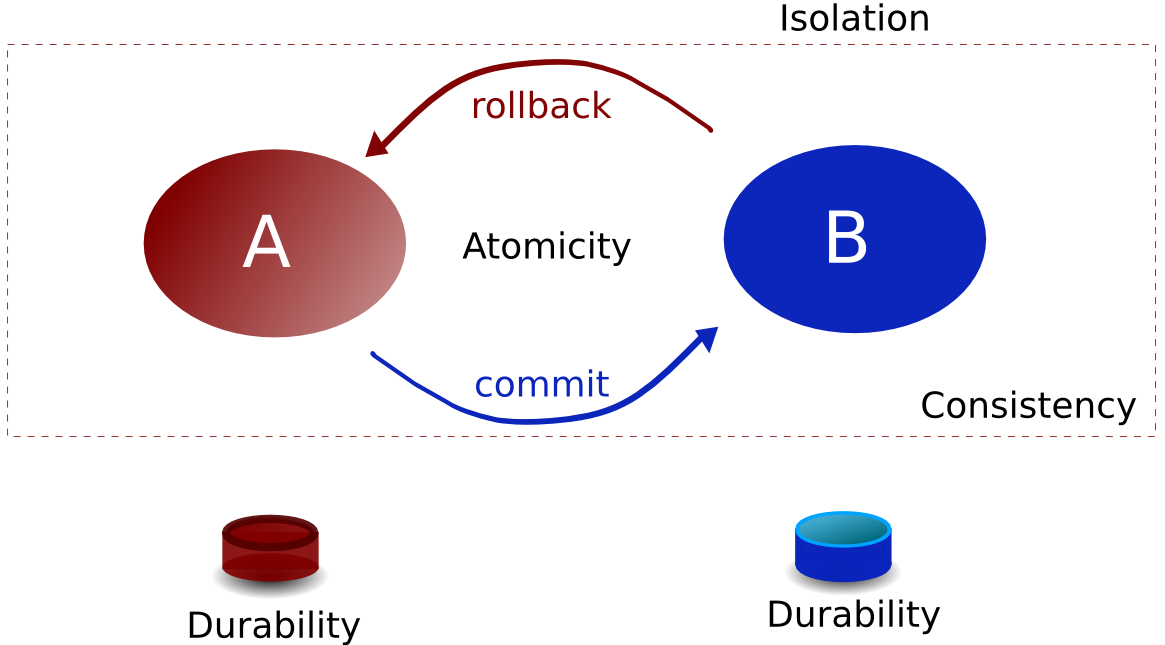
\includegraphics[scale=0.3]{img/transaction.png}
%--   \end{center}
%--  \end{frame}

\ifbook{
  \mysubsubsection{Rôle d'un cache}

  \paragraph{} Mettre en cache une donnée ou un résultat consiste à le ou la conserver dans une source
  de données plus facilement accessible que la source de l'information.
}

\ifslide{
  \begin{frame}{Cache sind über alles}
    \begin{center}
      \begin{block}{Différents caches}
        \begin{itemize}
          \item cache DNS
          \item cache du navigateur
          \item cache HTTP
          \item la session est un cache
          \item cache SQL %(Hibernate)
          \item cache applicatif
        \end{itemize}
      \end{block}
    \end{center}
  \end{frame}
}

% TODO: cache
% niveau de cache
%statégie de cache
